\documentclass[a4paper,12pt,titlepage]{scrartcl}
\usepackage[utf8]{inputenc}
\usepackage{graphicx}
\usepackage{listings}
\usepackage{xcolor}
\usepackage{titlepic}

\lstset{
    frame=tb, % draw a frame at the top and bottom of the code block
    tabsize=4, % tab space width
    showstringspaces=false, % don't mark spaces in strings
    numbers=left, % display line numbers on the left
    commentstyle=\color{green}, % comment color
    keywordstyle=\color{blue}, % keyword color
    stringstyle=\color{red} % string color
}


\title{NVS Projekt: Aufzugsteuerung}
\author{Ralf Kühmayer}
\date{January 2021}
\titlepic{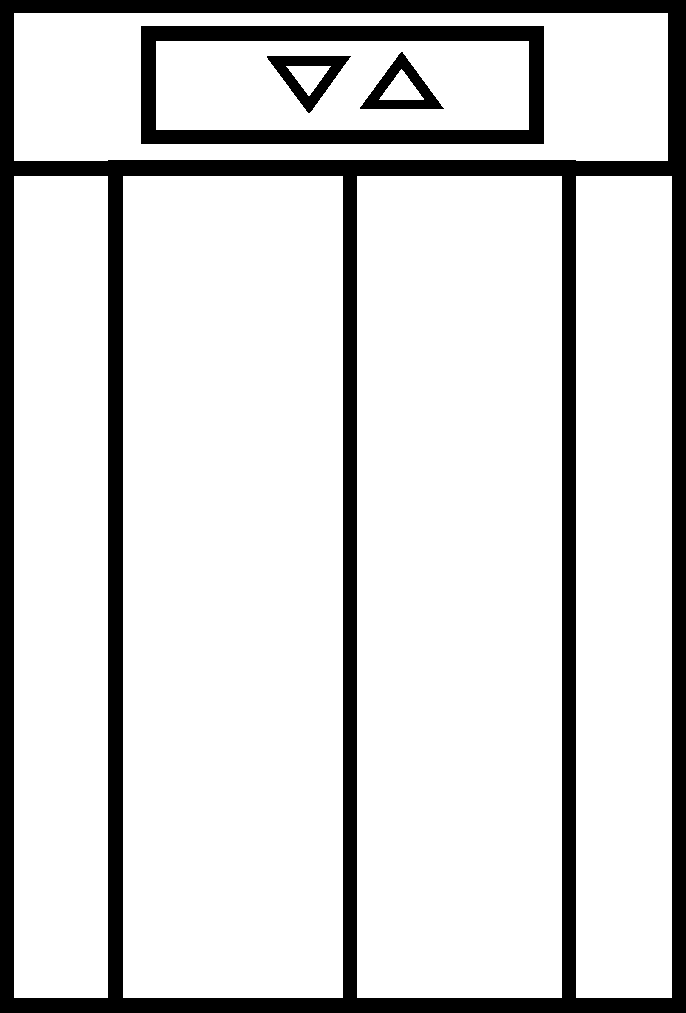
\includegraphics[width=60mm]{Elevator.pdf}}


\begin{document}

\maketitle

\newpage

\tableofcontents

\newpage

\section{Aufgabenstellung}

Ein kleines Beispiel für eine Aufzugssteuerung. Jedes Stockwerk und jeder Aufzug wird durch einen Thread repräsentiert. Es gibt einen zentralen Koordinator, der entscheidet, welcher Aufzug in welches Stockwerk fahren soll. In diesen Threads werden die in einem Aufzug oder einem Stockwerk gedrückten Knöpfe, um den Aufzug zu bewegen, vom Anwender simuliert. In der CLI gibt es Optionen, um auszuwählen, wie viele Aufzüge und Stockwerke simuliert werden. Es gibt auch Optionen für die Fahrzeit zwischen den Etagen und ob es die Möglichkeit eines Overrides in der CLI gibt. Des Weiteren kann in der CLI angegeben werden, dass eine Simulation anstelle des REPLs verwendet wird. Es gibt auch Optionen für logging und die Konfiguration kann auch durch eine JSON oder TOML Datei vorgenommen werden.


\section{Verwendung}
Das Programm wird durch den Aufruf von ./elevator\_control in der Kommandozeile gestartet. Beim Aufruf ohne Parameter startet das Programm mit 3 Stockwerken, 1 Aufzug und 3 Sekunden Fahrzeit zwischen den Stockwerken. Das Programm kann entweder durch die Eingabe des end Kommandos in das REPL beendet werden oder durch Abbruch mit Strg+c. Wird das Programm abgebrochen, wird es sofort geschlossen und die Aufzüge arbeiten ihre Queue nicht mehr ab. Wird das Programm jedoch mit dem end Kommando geschlossen, wartet das Programm noch solange, bis alle Aufzüge ihre Queue abgearbeitet haben, bevor es sich schließt.

\subsection{Parameter}
Das Programm hat einige optionale Parameter, mit welchen der Anwender das Programm Konfigurieren, das Logging ändern und die Bedienung des Programmes verändern kann.


\subsubsection{Programmparameter}
Programmparameter sind Parameter, welche das Verhalten oder Anzahlen in dem Programm beeinflussen.

\paragraph{-s, \texttt{-{}-}seconds-between-floors $<positive \: Kommazahl>$}\mbox{} \\
Mit dem Parameter -s oder \texttt{-{}-}seconds-between-floors und einer positiven Kommazahl kann der Anwender einstellen, wie lange ein Aufzug von einem Stockwerk zum nächstgelegenen Stockwerk in Sekunden braucht. Wenn der Parameter nicht angegeben wird, ist standardmäßig eine Fahrzeit von 3 Sekunden zwischen den Stockwerken festgelegt.

\paragraph{-f, \texttt{-{}-}floor-number $<positive \: ganze \: Zahl>$}\mbox{} \\
Mit dem Parameter -f oder \texttt{-{}-}floor-number und einer positiven ganzen Zahl kann der Anwender einstellen, wie viele Stockwerke es gibt. Wenn der Parameter nicht angegeben wird, sind standardmäßig 3 Stockwerke vorhanden.

\paragraph{-e, \texttt{-{}-}elevators $<positive \: ganze \: Zahl>$}\mbox{} \\
Mit dem Parameter -e oder \texttt{-{}-}elevators und einer positiven ganzen Zahl, kann der Anwender einstellen, wie viele Aufzüge es gibt. Wenn der Parameter nicht angegeben wird, ist standardmäßig nur ein Aufzug vohanden.

\paragraph{-o, \texttt{-{}-}override}\mbox{} \\
Mit dem Parameter -o oder \texttt{-{}-}override, wird eingestellt, dass die Befehle Move und Call auch mit einem override Flag ausgeführt werden können. Wir ein Befehl mit einem Override ausgeführt, hat das zur Folge, dass der ausgewählte Aufzug das angegebene Stockwerk als nächstes anzusteuerndes Stockwerk in seine Queue einfügt.

\subsubsection{Simmulationsparameter}
Simulationsparameter sind Parameter, mit welchen man das REPL durch eine Simulation ersetzen kann und diese damit auch konfiguriert.

\paragraph{\texttt{-{}-}simulation}\mbox{} \\
Wird der Parameter \texttt{-{}-}simulation gesetzt, dann wird das REPL durch eine Simulation ersetzt. Der Anwender kann diese Simulation durch eine Eingabe der Entertaste beenden, jedoch werden alle Aufzüge ihre Queue noch leeren und dann nach wird das Programm geschlossen.

\paragraph{\texttt{-{}-}simulation-time $<positive \: Kommazahl>$}\mbox{} \\
Mit dem Parameter \texttt{-{}-}simulation-time und einer positiven Kommazahl kann der Anwender einstellen, wie lange es nach einem Befehl dauert, bis der nächste Befehl gesendet wird.

\subsubsection{Konfigurationsparameter}
Konfigurationsparameter sind Parameter, welche durch eine angegebene Konfigurationsdatei die Programmparameter ersetzen. Es dürfen nicht beide Konfigurationsparameter gleichzeitig verwendet werden. Immer nur einer ohne Programmparameter.

\paragraph{-j, \texttt{-{}-}config-file-json $<Dateipfad>$}\mbox{} \\
Mit dem Parameter -j oder \texttt{-{}-}config-file-json und dem Pfad zu der Konfigurationsdatei kann angegeben werden, dass das Programm mit einer JSON-Datei konfiguriert werden soll. Wird dieser Parameter angegeben, darf kein Programmparameter verwendet werden, Simulations- und Loggingparameter können verwendet werden.

\paragraph{-t, \texttt{-{}-}config-file-toml $<Dateipfad>$}\mbox{} \\
Mit dem Parameter -t oder \texttt{-{}-}config-file-toml und dem Pfad zu der Konfigurationsdatei kann angegeben werden, dass das Programm mit einer TOML-Datei konfiguriert werden soll. Wird dieser Parameter angegeben, darf kein Programmparameter verwendet werden, Simulations- und Loggingparameter können verwendet werden.


\subsubsection{Loggingparameter}
Mit den Loggingparametern wird das Logging in eine Datei aktiviert und es kann dieses konfiguriert werden. Standardmäßig ist das Logginglevel auf Info gesetzt, das kann jedoch genau so wie die Datei konfiguriert werden.

\paragraph{-l, \texttt{-{}-}log-to-file}\mbox{} \\
Mit dem Parameter -l oder \texttt{-{}-}log-to-file, kann der Anwender einstellen, dass das Logging in eine Datei aktiviert wird. Das default Logginglevel ist Info und es wird standardmäßig in die Datei control.log in dem aktuellen Ordner geschrieben. Existiert diese Datei nicht, wird sie erstellt.

\paragraph{-d, \texttt{-{}-}log-level-debug}\mbox{} \\
Mit dem Parameter -d oder \texttt{-{}-}log-level-debug wird das Logginglevel, für das Loggen in eine Datei vom Level Info auf das Level Debug geändert. Dadurch werden mehr Informationen in der Logdatei gespeichert.

\paragraph{\texttt{-{}-}log-file $<Dateipfad>$}\mbox{} \\
Mit dem Parameter \texttt{-{}-}log-file und dem Pfad zu einer Datei kann die Datei spezifiziert werden, in welche der Logger schreiben soll. Wenn diese Datei bereits existiert, hängt der Logger seine Nachrichten einfach am Ende der Datei an. Existiert die Datei jedoch nicht, wird eine neue Datei erstellt.


\break

\section{Objekte}

\subsection{Stockwerk}

\begin{lstlisting}[language=C++]
class Floor
{
private:
    std::string name{"Floor"};
    unsigned int id{};
    MessageQueue* message_queue;
    MessageQueue* coordinator_queue;
    std::shared_ptr<spdlog::logger> file_logger;
    bool running{true};

public:
    Floor(unsigned int id
    , MessageQueue* coordinator_queue
    , std::shared_ptr<spdlog::logger> file_logger);
    void operator()();
    void push(Message message);
};
\end{lstlisting}

\vspace{5mm}

Das Stockwerk Objekt bekommt bei der Initialisierung eine ID, welche gleichzeitig die Nummer des Stockwerkes ist, die Nachrichtenqueue des Koordinators, um Nachrichten an den Koordinator zu schicken und einen shared Pointer für das Logging in eine Datei. Des Weiteren wird auch der Name auf Floor gesetzt. Mit dem Namen und der ID kann das Stockwerk eindeutig identifiziert werden. Des Weiteren hat ein Stockwerk auch einen eigene Nachrichtenqueue, in welche das Repl oder die Simulation Nachrichten stellen, welche von dem Stockwerk bearbeitet und an den Koordinator gesendet werden. Um diese Nachrichten in die Queue einzufügen, hat das Objekt eine öffentliche Methode push, welche eine Nachricht als Parameter benötigt. Die öffentliche Methode operator wird verwendet, um einen Thread für das Stockwerk zu starten. In dieser Methode wartet das Objekt auf eine Nachricht vom REPL oder der Simulation und wenn es eine Nachricht erhält, wird eine Ausgabe getätigt, die Nachricht verändert und an den Koordinator weiter gesendet. Die boolsche Variable running ist dafür da, dass der Thread so lange eine Schleife aufruft, um auf Nachrichten zu warten und sie weiter zu senden, bis eine Nachricht mit dem Befehl stop kommt. Dann wird diese Variable auf false gesetzt und der Thread schließt sich.

\break

\subsection{Aufzug}


\begin{lstlisting}[language=C++]
Class Elevator
{
private:
    std::string name{"Elevator"};
    unsigned int id{1};
    unsigned int current_floor{1};
    bool moving{false};
    float travel_time{3.0};
    MessageQueue* message_queue;
    MessageQueue* coordinator_queue;
    NextFloor_Queue* next_floors;
    std::shared_ptr<spdlog::logger> file_logger;

public:
    Elevator(unsigned int id, float travel_time
    , MessageQueue* coordinator_queue
    , std::shared_ptr<spdlog::logger> file_logger);
    void move_to(unsigned int floor);
    void first(unsigned int floor);
    unsigned int get_current_floor();
    bool is_moving();
    void operator()();
    void buttons();
    void push(Message message);
};
\end{lstlisting}

\vspace{5mm}

Ein Aufzug bekommt bei der Initialisierung einen Namen, eine ID, in welchem Stock er sich gerade befindet, die Fahrzeit, die er zwischen zwei Stockwerken benötigt, die Koordinatorqueue, an welche er Nachrichten sendet und einen shared Pointer für das Logging in eine Datei. Durch den Namen und die ID kann jeder Aufzug eindeutig identifiziert werden. Des Weiteren erstellt er bei der Initialisierung eine Nachrichtenqueue, in welche mit der öffentlichen Methode push eine Nachricht eingefügt werden kann. Ebenfalls wird eine Aufzugsqueue erstellt, in diese Queue wird mit den öffentlichen Methoden first und move\_to etwas eingefügt, beide Methoden brauchen eine positive ganze Zahl als Parameter. Die Methode first wird nur dann aufgerufen, wenn ein Befehl mit einem Override Flag versehen wurde, dadurch werden alle Elemente, die gerade in der Aufzugsqueue sind, nach hinten verschoben und das übergebene Stockwerk wird an erster Stelle eingefügt. Bei der Methode move\_to wird zu erst überprüft, ob das Stockwerk zwischen dem Aktuellen und dem Nächsten liegt, dann wird es als Erstes in die Aufzugsqueue eingefügt, ansonsten wird es an die Queue übergeben, um es an einer passenden Stelle einzufügen. Diese beiden Methoden werden nur von dem Koordinator aufgerufen. Damit der Koordinator weiß, ob sich ein Aufzug gerade bewegt oder nicht, hat ein Aufzug die Methode is\_moving, welche true zurückgibt, wenn er sich bewegt, und wenn er gerade in einem Stockwerk steht, wird flase zurückgegeben. Aus einem Aufzugsobjekt werden zwei Threads erstellt. Der erste Thread ruft die Methode buttons auf.  Diese Methode wartet auf Nachrichten vom REPL oder der Simulation, bearbeitet diese und gibt sie an den Koordinator weiter. Dadurch wird das Drücken eines Knopfes in einem Aufzug simuliert. Diese Methode führt das warten, bearbeiten, senden so lange in einer Schleife aus, bis eine Nachricht mit dem Kommando stop erfolgt. Erfolgt diese Nachricht, sendet das Objekt die Nachricht mit dem stop Kommando weiter an den Koordinator und beendet sich danach. Die Methode operator hingegen simuliert die Bewegungen des Aufzuges. Es wird in einer Schleife überprüft, ob man das Ziel erreicht hat, ob es ein neues Ziel gibt oder ob überhaupt noch Ziele in der Queue sind. Hat der Aufzug sein Ziel erreicht, gibt er eine Nachricht aus und löscht dieses Element aus seiner Queue. Wenn sich nach dem Löschvorgang keine Ziele mehr in der Queue befinden, setzt er die Variable moving auf false. Jedes Mal, wenn ein Aufzug sein Ziel erreicht, wartet er auf diesem Stockwerk eine Sekunde, was das Ein- und Aussteigen von Personen simulieren soll. Danach wartet er, bis das nächste Ziel in der Queue ist. Ist die Queue noch nicht leer, holt er sich das nächste Ziel und überprüft, ob es dem Zeichen für stop entspricht. Entspricht es diesem Zeichen, beendet sich der Thread. Entspricht es jedoch nicht dem Zeichen, dann wird die Variable moving auf true gesetzt und der Aufzug fährt weiter. Es wird auch überprüft, ob sich das nächste Ziel in der Zwischenzeit geändert hat und falls es sich geändert hat, in der lokalen Variable die Änderung als neues Ziel gesetzt.

\subsection{Koordinator}

\begin{lstlisting}[language=C++]
class Coordinator
{
private:
    std::vector<Elevator>& elevators;
    MessageQueue* message_queue;
    std::string name{"Coordinator"};
    std::shared_ptr<spdlog::logger> file_logger;
    unsigned int get_closest_elevator(Message message);
    
public:
    Coordinator(std::vector<Elevator>& elevators
    , MessageQueue* message_queue
    , std::shared_ptr<spdlog::logger> file_logger);
    void operator()();
};
\end{lstlisting}

\vspace{5mm}

Ein Koordinator bekommt bei der Initialisierung alle Aufzüge, seine Nachrichtenqueue und den shared Pointer für das Logging in eine Datei. Der Koordinator wird mit der Methode operator in einem Thread gestartet und wartet auf Nachrichten von einem Aufzug oder einem Stockwerk in seine Nachrichtenqueue. Wenn er eine Nachricht bekommt, muss er das Kommando auslesen. Ist das Kommando ein Override dann wird die boolsche Variable für override auf true gesetzt und danach aufgrund der Aufzugsid geschaut, ob ein Call Kommando oder ein Move Kommando mit Override aufgerufen wurde. Das kann dadurch erreicht werden, da bei einem Call die Aufzugsid immer 0 ist, es aber keinen Aufzug mit dieser ID gibt. Ist es ein Kommando ohne Override, dann kann die Art des Kommandos einfach ausgelesen werden. Ist es ein Move Kommando wird in die Aufzugqueue des Aufzuges, in welchem der Knopf gedrückt wurde, das Stockwerk eingefügt. Wenn es ein Override Kommando war mit der Methode first des Aufzuges ansonsten mit der Methode move\_to. Ist das Kommando jedoch kein Move, sondern ein Call, muss der Koordinator zuerst schauen, welcher Aufzug sich bewegt und welcher am nächsten ist. Das erfolgt durch die private Methode get\_closest\_elevator. Diese Methode ruft die statischen Methoden closest\_elevator\_not\_mooving und closest\_elevator\_with\_mooving auf. Diese Methoden werden asynchron in einem eigenen Thread gestartet und durch ein future-promis-paar wird das Ergebnis abgefragt. Es wird zuerst überprüft, ob sich ein Aufzug nicht bewegt, wenn das der Fall ist, wird der nächste sich nicht bewegende Aufzug ausgesucht. Bewegen sich jedoch alle Aufzüge, wird der Aufzug ausgesucht, der sich dem Stockwerk am nähesten befindet. Steht der Aufzug jetzt fest, so wird wie bei einem Move das Stockwerk in die Aufzugsqueue des Aufzuges eingefügt. Bei einem Override wieder mit der Methode first und wenn es kein override ist mit der Methode move\_to.

\subsection{REPL (Read–eval–print loop)}

\begin{lstlisting}[language=C++]
class Repl
{
private:
    std::vector<Floor>& floors;
    std::vector<Elevator>& elevators;
    unsigned int floor_number{};
    unsigned int elevator_number{};
    bool override{false};
    bool use_simulation{false};
    bool& running;
    std::shared_ptr<spdlog::logger> file_logger;
    void move(std::string floor_number
    , std::string elevator_number, bool override);
    void call(std::string number, bool override);
    void show_help();
    void stop();

public:
    Repl(std::vector<Floor>& floors
    , std::vector<Elevator>& elevators
    , unsigned int floor_number
    , unsigned int elevator_number, bool override
    , std::shared_ptr<spdlog::logger> file_logger
    , bool use_simulation, bool& running);
    void operator()();
};
\end{lstlisting}

\vspace{5mm}

Das REPL oder Read–eval–print loop ist eine Schleife, die Anwendereingaben list diese evaluiert, danach etwas ausgibt und das ganze in einer Schleife solange macht, bis der Anwender es abbricht oder das end Kommando eingibt. Bei der Initialisierung des REPLs werden alle Stockwerke, alle Aufzüge, die Anzahl der Stockwerke, die Anzahl der Aufzüge, ob override aktiv ist, der shared Pointer für das Logging in die Datei, ob die Simulation aktiv ist und ob das Programm läuft übergeben. Zuerst wird überprüft, ob eine Simulation läuft und wenn eine Simulation läuft, wird nur auf eine Eingabe gewartet, damit die Variable running auf false gesetzt werden kann uns somit die Simulation weiß, dass das Programm beendet wurde. Ist die Simulation jedoch nicht aktiv, wird zuerst die Grammatik für das REPL definiert. Dabei wird überprüft, ob Override aktiv ist. Ist es Aktiv wird es in die Grammatik eingebunden, ist es nicht aktiv, gilt die Eingabe eines Override Kommando als Fehler. Nachdem die Grammatik definiert ist, startet die Schleife. In dieser Schleife wird auf eine Eingabe des Anwenders gewartet. Ist eine Eingabe vorhanden, wird diese mit der Grammatik verglichen. Dadurch werden nicht vorhanden Kommandos ignoriert und es wird eine Information für den Anwender angezeigt, dass seine Eingabe keinem Kommando entspricht und welche Kommandos es gibt. Ist das Kommando jedoch als gültig erklärt worden, dann wird überprüft, um welches Kommando es sich handelt. Handelt es sich um das Kommando help, wird eine Infonachricht mit allen verfügbaren Kommandos ausgegeben. Handelt es sich um einen Override Kommando, wird eine lokale boolsche Variable auf true gesetzt und override wird aus dem string gelöscht, um in weiter zu überprüfen. Danach wird unterschieden zwischen einem call und einem move befehl. Bei einem Call befehl wird danach eine Zahl für die Stockwerksnummer angegeben, diese Muss von einem String zu einer ganzzahligen positiven Zahl konvertiert werden. Ist das erledigt, wird die Methode call aufgerufen. Diese Methode überprüft, ob es überhaupt soviel Stockwerke gibt, wie vom Anwender angegeben. Gibt es nicht so viele Stockwerke, wird eine Warnung ausgegeben mit der Anzahl der existierenden Stockwerke und der vom Anwender eingegebenen Anzahl. Ist die angegebene Zahl im Bereich des Möglichen, wird noch überprüft, ob override verwendet wurde, also dass die Variable true ist und dann die dementsprechende Nachricht an das dementsprechende Stockwerk geschickt. Ist es kein Call Kommando, sonder ein Move Kommando, müssen zwei Zahlen konvertiert werden und es wird die Methode move aufgerufen. Diese Methode überprüft ebenfalls, ob die eingegebene Zahl für das Stockwerk und die eingegebene Zahl für den Aufzug im Bereich des Möglichen sind. Sind sie es nicht, wird eine Warnung ausgegeben, mit wie viele Aufzüge oder Stockwerke es gibt und was ihre Eingabe war. Ist die Eingabe jedoch korrekt, wird überprüft, ob override verwendet wurde, also dass die Variable true ist und dann die dementsprechende Nachricht an den dementsprechenden Aufzug geschickt. Wird das Kommando end eingegeben, sendet das REPL an alle Aufzüge und an alle Stockwerke die Nachricht stop. Außerdem setzt es die Variable running auf flase und beendet somit die Schleife und den Thread.

\subsection{Simulation}

\begin{lstlisting}[language=C++]
class Simulation
{
private:
    std::vector<Floor>& floors;
    std::vector<Elevator>& elevators;
    bool override{false};
    bool& running;
    std::shared_ptr<spdlog::logger> file_logger;
    float sim_time{};
    unsigned int floor_number{};
    unsigned int elevator_number{};
    void move(unsigned int floor_number
    , unsigned int elevator_number, bool override);
    void call(unsigned int number, bool override);

public:
    Simulation(std::vector<Floor>& floors
    , std::vector<Elevator>& elevators
    , unsigned int floor_number
    , unsigned int elevator_number, bool override
    , std::shared_ptr<spdlog::logger> file_logger
    , float sim_time, bool& running);
    void operator()();
};
\end{lstlisting}

\vspace{5mm}

Die Simulation benötigt bei Initialisierung alle Stockwerke, alle Aufzüge, die Anzahl der Stockwerke, die Anzahl der Aufzüge, ob es override gibt oder nicht, den shared Pointer für das Logging in eine Datei, die Zeit zwischen den Kommandos und ob die Simulation beendet ist. Die Simulation wird mit der Methode operator als Thread gestartet. Es wird eine Schleife ausgeführt, die zufällig ein Kommando generiert, wenn override aktiv ist auch override Kommandos. Diese Kommandos werden dann mit den privaten Methoden move und call weiter bearbeitet. Wenn ein call Kommando mit einer Stockwerksnummer generiert wurde, wird die Methode call aufgerufen, um dieses Kommando in eine Nachricht zu verpacken und es an das dementsprechende Stockwerk zu schicken. Bei einem Move Kommando wird die Methode move aufgerufen, um dieses generierte Kommando in eine Nachricht zu verpacken und an den dementsprechenden Aufzug zu verschicken. Wird ein override Kommando, generiert wir einfach eine boolsche Variable auf true gesetzt und beide Methoden setzten dieses Kommando in die Nachricht ein. Die Simulation läuft solange, bis eine Anwendereingabe das Programm beendet. Das wird durch die boolsche Variable running realisiert, welche bei einer Anwendereingabe auf false gesetzt wird.

\subsection{Aufzugsqueue}

\begin{lstlisting}[language=C++]
class NextFloor_Queue
{
private:
    std::vector<unsigned int> next_floors{};
    std::mutex m{};
    std::condition_variable con_empty{};
    std::shared_ptr<spdlog::logger> file_logger;

public:
    NextFloor_Queue
        (std::shared_ptr<spdlog::logger> file_logger);
    unsigned int front();
    unsigned int get();
    void erase(unsigned int floor);
    void insert_first(unsigned int floor);
    void insert(unsigned int floor);
    bool empty();

};
\end{lstlisting}

\vspace{5mm}

Die Aufzugsqueue bekommt bei der Initialisierung den shared Pointer für das Logging in Dateien und es wird ein Vector angelegt, welcher positive ganze Zahlen speichern kann. Um in diesen Vector etwas einfügen zu können, gibt es zwei öffentliche Methoden, insert\_first und insert. Beide Methoden benötigen als Parameter eine positive ganze Zahl. Der Unterschied dieser beiden Methoden ist das insert\_first den Parameter immer als Erstes einfügt. Wohingegen insert den Parametern nach seinem numerischen Wert einordnet. Um aus diesem Vector auch wieder etwas auslesen zu können, gibt es die Methoden first und get. Bei der Methode first wird der erste Wert des Vectors zurückgegeben und wenn keiner existiert 0. Bei get wird ebenfalls der erste Wert zurückgegeben, existiert aber kein wert, dann wird gewartet, bis einer eingefügt wird. Des Weiteren gibt es noch die Methode erase um einen Wert aus dem Vector zu löschen und die Methode empty die zurückgibt, ob der Vector leer ist oder nicht.

\subsection{Nachrichtenqueue}

\begin{lstlisting}[language=C++]
class MessageQueue
{
private:
    std::queue<Message> message_queue{};
    std::mutex m{};
    std::condition_variable empty{};
    
public:
    Message pop();
    void push(Message message);
};
\end{lstlisting}

\vspace{5mm}

Die Nachrichtenqueue ist die direkte Kommunikationsverbindung zwischen den Aufzugsthreads, den Stockwerk Threads, dem Koordinator Thread und dem REPL Thread oder dem Simulationsthread. Bei der Initialisierung muss nichts übergeben werden. Des Weiteren enthält die Nachrichtenqueue eine Queue, welche Objekte vom Typ Nachricht speichern kann. Damit auf diese Queue zugegriffen werden kann, gibt es die öffentlichen Methoden pop und push. Bei der Methode pop wird die nächste Nachricht aus der Queue geholt, aus der Queue gelöscht und zurück übergeben. Ist keine Nachricht in der Queue vorhanden, wird gewartet, bis eine eingefügt wird. Mit push fügt man eine Nachricht in die Queue ein und benachrichtigt das wartende pop.

\subsection{Nachricht}

\begin{lstlisting}[language=C++]
class Message
{
private:
    std::string message{};
    std::string command{};
    unsigned int floor{};
    unsigned int elevator_id{};
    
public:
    Message(std::string message, std::string command
    , unsigned int floor, unsigned int elevator_id);
    std::string get_message();
    std::string get_command();
    unsigned int get_floor();
    unsigned int get_elevator_id();
    std::string to_string();
};
\end{lstlisting}

\vspace{5mm}

Eine Nachricht wird verwendet, um zwischen den Stockwerken, den Aufzügen, dem Koordinator und dem REPL oder der Simulation eine einheitliche Kommunikationsbasis herzustellen. Beim Initialisieren einer Nachricht müssen eine Nachricht, ein Kommando, eine Stockwerknummer und eine Aufzugsid übergeben werden. Für jedes dieser Attribute gibt es eine Funktion, um ihren Wert Auslesen zu können.

\section{Programmstart}

Bei Programmstart werden zuerst alle Parameter überprüft und die dazu Angegebenen Werte des Benutzers. Ist irgend ein Wert nicht korrekt oder fehlerhaft, wird eine Info an den Benutzer ausgegeben und das Programm geschlossen. Danach wird überprüft, ob eine Konfigurationsdatei verwendet wird. Wird eine solche verwendet, wird diese validiert und die Werte werden übertragen. Ist die Datei jedoch nicht Valide, also sie weißt Fehler auf, wird ebenfalls eine Info an den Benutzer ausgegeben und das Programm beendet. Die nächste Überprüfung ist, ob das Loggen in eine Datei aktiviert wurde und welches Logginglevel verwendet werden soll. Dieser Logger wird erstellt und auf das Logginglevel konfiguriert. Des Weiteren wird das Pattern, mit welchem der Logger schreiben soll, für die Kommandozeilenausgabe genauso wie für das Logging in eine Datei konfiguriert. Der nächste Schritt ist das VeKtoren für die Stockwerke, die Aufzüge und die Threads erstellt werden. Diese Vektoren reservieren sich dann den Speicherplatz, den sie brauchen werden. Als Nächstes wird eine Ausgabe getätigt, welche den Status des Programmes ausgibt, also wie viele Aufzüge es gibt, ob Logging aktiviert ist und so weiter. Die nächste Überprüfung ist, ob der Benutzer die Simulation eingeschalten hat oder ob er das Programm per REPL bedienen will. Je nachdem wird eine Nachricht ausgegeben bei der Simulation, wie man sie beendet, beim REPL wie man die Hilfe aufruft. Als Nächstes werden die Threads für die Stockwerke, die Aufzugsbewegungen, die Aufzugsnachrichten, den Koordinator, das REPL und wenn aktiviert auch für die Simulation erstellt und gestartet. Mit dem Starten der Threads wird der Programmfluss an die Threads abgegeben und es wird nur noch gewartet, bis sich die Threads beenden. Nachdem alle Threads beendet sind, wird ausgegeben, dass das Programm sich beendet hat.

\end{document}